% Created 2021-12-19 Sun 10:05
\documentclass[9pt, b5paper]{article}
\usepackage[UTF8]{ctex}
\usepackage{xltxtra}
\usepackage{bera}
\usepackage[T1]{fontenc}
\usepackage[scaled]{beraserif}
\usepackage[scaled]{berasans}
\usepackage[scaled]{beramono}
\usepackage{graphicx}
\usepackage{xcolor}
\usepackage{multirow}
\usepackage{multicol}
\usepackage{float}
\usepackage{textcomp}
\usepackage{geometry}
\geometry{left=1.2cm,right=1.2cm,top=1.5cm,bottom=1.2cm}
\usepackage{algorithm}
\usepackage{algorithmic}
\usepackage{latexsym}
\usepackage{natbib}
\usepackage{minted}
\newminted{common-lisp}{fontsize=ootnotesize}
\usepackage[xetex,colorlinks=true,CJKbookmarks=true,linkcolor=blue,urlcolor=blue,menucolor=blue]{hyperref}
\author{deepwaterooo}
\date{\today}
\title{Android Study Plan}
\hypersetup{
  pdfkeywords={},
  pdfsubject={},
  pdfcreator={Emacs 27.1 (Org mode 8.2.7c)}}
\begin{document}

\maketitle
\tableofcontents


\section{性能优化}
\label{sec-1}
\begin{itemize}
\item \url{https://segmentfault.com/a/1190000037449196} 总结得很全面也很透彻
\end{itemize}
\subsection{内存优化}
\label{sec-1-1}
\subsubsection{珍惜Service,尽量使得Service在使用的时候才处于运行状态。尽量使用IntentService}
\label{sec-1-1-1}
\begin{itemize}
\item IntentService在内部其实是通过线程以及Handler实现的,当有新的Intent到来的时候,会创建线程并且处理这个Intent,处理完毕以后就自动销毁自身。因此使用IntentService能够节省系统资源。
\end{itemize}
\subsubsection{内存紧张的时候释放资源(例如UI隐藏的时候释放资源等)。复写Activity的回调方法。}
\label{sec-1-1-2}
\begin{minted}[frame=lines,fontsize=\scriptsize,linenos=false]{java}
@Override 
public void onLowMemory() { 
    super.onLowMemory(); 
}  
@Override 
public void onTrimMemory(int level) { 
    super.onTrimMemory(level);  
    switch (level) { 
    case TRIM_MEMORY_COMPLETE: 
        break; 
    case 其他: 
    } 
}
\end{minted}
\subsubsection{通过Manifest中对Application配置更大的内存,但是一般不推荐}
\label{sec-1-1-3}
\begin{minted}[frame=lines,fontsize=\scriptsize,linenos=false]{xml}
android:largeHeap="true"
\end{minted}
\subsubsection{避免Bitmap的浪费,应该尽量去适配屏幕设备。尽量使用成熟的图片加载框架,Picasso,Fresco,Glide等。}
\label{sec-1-1-4}
\subsubsection{使用优化的容器,SparseArray等}
\label{sec-1-1-5}
\begin{itemize}
\item Android为什么推荐使用SparseArray来替代HashMap?
\item SparseArray有两个优点:
\begin{itemize}
\item 1.避免了自动装箱(auto-boxing)
\item 2.数据结构不会依赖于外部对象映射。我们知道HashMap 采用一种所谓的“Hash 算法”来决定每个元素的存储位置,存放的都是数组元素的引用,通过每个对象的hash值来映射对象。而SparseArray则是用数组数据结构来保存映射,然后通过折半查找来找到对象。但其实一般来说,SparseArray执行效率比HashMap要慢一点,因为查找需要折半查找,而添加删除则需要在数组中执行,而HashMap都是通过外部映射。但相对来说影响不大,最主要是SparseArray不需要开辟内存空间来额外存储外部映射,从而节省内存。
\end{itemize}
\end{itemize}
\subsubsection{其他建议:尽量少用枚举变量,尽量少用抽象,尽量少增加类,避免使用依赖注入框架,谨慎使用library,使用代码混淆,时当场合考虑使用多进程等。}
\label{sec-1-1-6}
\subsubsection{避免内存泄漏(本来应该被回收的对象没有被回收)}
\label{sec-1-1-7}
\begin{itemize}
\item 一旦APP的内存短时间内快速增长或者GC非常频繁的时候,就应该考虑是否是内存泄漏导致的。
\end{itemize}
\begin{enumerate}
\item 什么情况会导致内存泄漏
\label{sec-1-1-7-1}
\begin{itemize}
\item 1.资源释放问题:程序代码的问题,长期保持某些资源,如Context、Cursor、IO 流的引用,资源得不到释放造成内存泄露。 
\begin{itemize}
\item 资源对象没有关闭引起的内存泄漏。在这些资源不使用的时候,记得调用相应的类似close()、destroy()、recycler()、release()等方法释放。
\item 注册/反注册未成对使用引起的内存泄漏。注册广播接受器、EventBus等,记得解绑。
\end{itemize}
\item 2.对象内存过大问题:保存了多个耗用内存过大的对象(如Bitmap、XML 文件),造成内存超出限制。
\item 3.static 关键字的使用问题:static 是Java 中的一个关键字,当用它来修饰成员变量时,那么该变量就属于该类,而不是该类的实例。所以用static 修饰的变量,它的生命周期是很长的,如果用它来引用一些资源耗费过多的实例(Context 的情况最多),这时就要谨慎对待了。
\begin{itemize}
\item 解决方案
\begin{itemize}
\item 应该尽量避免static 成员变量引用资源耗费过多的实例,比如Context。
\item Context 尽量使用ApplicationContext,因为Application 的Context 的生命周期比较长,引用它不会出现内存泄露的问题。
\item 使用WeakReference 代替强引用。比如可以使用WeakReference<Context> mContextRef
\end{itemize}
\end{itemize}
\item 4.线程导致内存溢出:线程产生内存泄露的主要原因在于线程生命周期的不可控。例如Activity中的Thread在run了,但是Activity由于某种原因重新创建了,但是Thread仍然会运行,因为run方法不结束的话Thread是不会销毁的。
\begin{itemize}
\item Handler 引起的内存泄漏。解决:将Handler声明为静态内部类,就不会持有外部类SecondActivity的引用,其生命周期就和外部类无关,如果Handler里面需要context的话,可以通过弱引用方式引用外部类
\item 解决方案
\begin{itemize}
\item 将线程的内部类,改为静态内部类(因为非静态内部类拥有外部类对象的强引用,而静态类则不拥有)。
\item 在线程内部采用弱引用保存Context 引用。
\end{itemize}
\end{itemize}
\end{itemize}
\item 内存泄漏的分析工具与方法
\label{sec-1-1-7-2}
\begin{itemize}
\item 使用Android Studio提供的Android Monitors中Memory工具查看内存的使用以及没使用的情况。
\item 使用DDMS提供的Heap工具查看内存使用情况,也可以手动触发GC。
\item 使用性能分析的依赖库,例如Square的LeakCanary,这个库会在内存泄漏的前后通过Notification通知你。
\end{itemize}
\begin{enumerate}
\item LeakCanary原理:
\label{sec-1-1-7-2-1}
\begin{itemize}
\item 它的基本工作原理如下:
\begin{itemize}
\item RefWatcher.watch() 创建一个 KeyedWeakReference 到要被监控的对象。
\item 然后在后台线程检查引用是否被清除,如果没有,调用GC。
\item 如果引用还是未被清除,把 heap 内存 dump 到 APP 对应的文件系统中的一个 .hprof 文件中。
\item 在另外一个进程中的 HeapAnalyzerService 有一个 HeapAnalyzer 使用HAHA 解析这个文件。
\item 得益于唯一的 reference key, HeapAnalyzer 找到 KeyedWeakReference,定位内存泄漏。
\item HeapAnalyzer 计算 到 GC roots 的最短强引用路径,并确定是否是泄漏。如果是的话,建立导致泄漏的引用链。
\item 引用链传递到 APP 进程中的 DisplayLeakService, 并以通知的形式展示出来。
\end{itemize}
\end{itemize}
\item 总的来说,LeakCanary有如下几个明显优点:
\label{sec-1-1-7-2-2}
\begin{itemize}
\item 针对Android Activity组件完全自动化的内存泄漏检查。
\item 可定制一些行为(dump文件和leaktrace对象的数量、自定义例外、分析结果的自定义处理等)。
\item 集成到自己工程并使用的成本很低。
\item 友好的界面展示和通知。
\end{itemize}
\end{enumerate}
\end{enumerate}

\subsection{性能优化}
\label{sec-1-2}
\begin{itemize}
\item 防止过度绘制,通过打开手机的“显示过度绘制区域”即可查看过度绘制的情况。
\item 最小化渲染时间,使用视图树查看节点,对节点进行性能分析。
\item 通过TraceView进行数据的采集以及分析。在有大概定位的时候,使用Android官方提供的Debug类进行采集。***通过DDMS即可打开这个.trace文件,分析函数的调用情况(包括在指定情况下执行时间,调用次数)
\end{itemize}
\begin{minted}[frame=lines,fontsize=\scriptsize,linenos=false]{java}
  // 开启数据采集 
  Debug.startMethodTracing("test.trace"); 
  // 关闭 
  Debug.stopMethodTracing();
\end{minted}

\subsection{OOM}
\label{sec-1-3}
\begin{itemize}
\item 避免OOM的一些常见方法:
\begin{itemize}
\item 1. App资源中尽量少用大图。使用Bitmap的时候要注意等比例缩小图片,并且注意Bitmap的回收。
\end{itemize}
\end{itemize}
\begin{minted}[frame=lines,fontsize=\scriptsize,linenos=false]{java}
 BitmapFactory.Options options = new BitmapFactory.Option(); 
 options.inSampleSize = 2; 
 //Options 只保存图片尺寸大小,不保存图片到内存 
 BitmapFactory.Options opts = new BitmapFactory.Options(); 
 opts.inSampleSize = 2; 
 Bitmap bmp = null; 
 bmp = BitmapFactory.decodeResource(getResources(), 
 mImageIds[position],opts); 
 //回收 
 bmp.recycle();
\end{minted}
\begin{itemize}
\item 2. 结合组件的生命周期,释放资源
\item 3. IO流,数据库查询的游标等应该在使用完之后及时关闭。
\item 4. ListView中应该使用ViewHolder模式缓存ConverView
\item 5. 页面切换的时候尽量去传递(复用)一些对象
\end{itemize}

\subsection{ANR}
\label{sec-1-4}
\begin{itemize}
\item 不同的组件发生ANR 的时间不一样,主线程(Activity、Service)是5 秒,BroadCastReceiver 是10 秒。
\item ANR一般有三种类型:
\begin{itemize}
\item 1. KeyDispatchTimeout(5 seconds)
\begin{itemize}
\item 主要类型按键或触摸事件在特定时间内无响应
\end{itemize}
\item 2. BroadcastTimeout(10 seconds)
\begin{itemize}
\item BroadcastReceiver在特定时间内无法处理完成
\end{itemize}
\item 3. ServiceTimeout(20 seconds)
\begin{itemize}
\item 小概率类型Service在特定的时间内无法处理完成
\end{itemize}
\end{itemize}
\item 解决方案:
\begin{itemize}
\item 1. UI线程只进行UI相关的操作。所有耗时操作,比如访问网络,Socket 通信,查询大量SQL 语句,复杂逻辑计算等都放在子线程中去,然后通过handler.sendMessage、runonUITread、AsyncTask 等方式更新UI。
\item 2. 无论如何都要确保用户界面操作的流畅度。如果耗时操作需要让用户等待,那么可以在界面上显示进度条。
\item 3. BroadCastReceiver要进行复杂操作的的时候,可以在onReceive()方法中启动一个Service来处理。
\end{itemize}
\end{itemize}
\subsection{内存抖动}
\label{sec-1-5}
\begin{itemize}
\item Gc 引起卡顿+OOM,怎么优化
\item Gson反序列化导致产生大量对象
\item 解决思考:对象池
\end{itemize}

\subsection{网络请求优化}
\label{sec-1-6}
\begin{itemize}
\item 能够缓存起来的尽量去缓存起来,减轻服务器的压力。例如APP中首页的一些数据,又例如首页的图标、文案都是缓存起来的,而且这些数据通过网络来指定可以使app具有更大的灵活性。
\item 不用域名,用 IP 直连,省去了DNS域名解析。
\item 连接复用、请求合并、请求数据Body可以利用压缩算法Gzip来进行压缩,使用JSON 代替 XML
\item 网络请求的安全性: 这块了解的不多。我给你说说我的思路吧,利用哈希算法,比如MD5,服务器给我们的数据可以通过时间戳和其他参数做个加密,得到一个key,在客户端取出数据后根据数据和时间戳再去生成key与服务端给的做个对比。
\end{itemize}

\section{app优化 (项目中处理的一些难点)}
\label{sec-2}
\begin{itemize}
\item 主要分为 启动优化,布局优化 ,打包优化 等
\end{itemize}
\subsection{启动优化}
\label{sec-2-1}
\begin{itemize}
\item 闪屏页 优化,设置theme 默认欢迎背景
\item 懒加载 第三方库,不要都放在application 中初始化
\item 如果项目中有 webview ,可以提前在app空闲时间加载 webview 的内核,如果多处使用 可以创建缓存池,缓存webview,
\item 如果android 5.0- 在applicaton 的 attchbaseContext() 中加载MultiDex.install 会更加耗时,可以采用 子线程(子线程加载 需要担心ANR 和ContentProvider 未加载报错的问题)或者单独开一个进程B,进程B开启子线程运行MultiDex.install ,让applicaton 进入while 循环等待B进程加载结果。
\item MultiDex 优化,apk打包分为 android 5.0 + 使用 ART虚拟机 不用担心
\end{itemize}
\subsection{布局UI优化}
\label{sec-2-2}
\begin{itemize}
\item 看过布局绘制源码流程后,可以知道 setContextView中 在ViewRootImpl 中使用 pull 的方法(这里可以扩展xml读取方式 SAX :逐行解析、dom:将整个文件加载到内存 然后解析,不推荐、pull:类似于 SAX 进行了android平台的优化,更加轻量级 方便)迭代读取 xml标签,然后对view 进行 measure,layout 和draw 的时候都存在耗时。通常优化方式有:
\begin{itemize}
\item 减少UI层级、使用merge、Viewstub标签 优化重复的布局
\item 优化 layout ,尽量多使用ConstraintLayout,因为 relalayout 和 linearlayout 比重的情况下都存在多次测量
\item recyclerView 缓存 ( 可扩展 说明 rv的缓存原理 )
\item 比较极端的 将 measure 和 layout 放在子线程,在主线程进行draw。或者 子线程中 加载view 进行IO读取xml,通过Handler 回调主线程 加载view(比如android 原生类 AsyncLayoutInflate )
\item 将xml直接通过 第三方工具(原理 APT 注解 翻译xml)直接将xml 转为 java代码
\end{itemize}
\end{itemize}


\section{数据交互}
\label{sec-3}
\subsection{Android中数据常见存储方式}
\label{sec-3-1}
\begin{itemize}
\item 文件(包括XML、SharePreference等)
\item 数据库
\item Content Provider
\item 保存在网络
\end{itemize}
\subsection{进程间通信}
\label{sec-3-2}
\subsubsection{操作系统进程间通信的方法,android中有哪些?}
\label{sec-3-2-1}
\begin{itemize}
\item Windows:剪贴板、管道、邮槽等
\item Linux:命名管道、共享内存、信号量
\end{itemize}
\subsubsection{Android中的进程通信方式并不是完全继承于Linux:}
\label{sec-3-2-2}
\begin{itemize}
\item Android 跨进程通信,像intent,contentProvider,广播,service都可以跨进程通信。
\begin{itemize}
\item intent:这种跨进程方式并不是访问内存的形式,它需要传递一个uri,比如说打电话。
\item contentProvider:这种形式,是使用内存映射、数据共享的形式进行数据共享。
\item service:远程服务,aidl
\end{itemize}
\item Intent 、Bundle : 要求传递数据能被序列化,实现 Parcelable、Serializable ,适用于四大组件通信。
\item 文件共享 :适用于交换简单的数据实时性不高的场景。
\item AIDL:AIDL 接口实质上是系统提供给我们可以方便实现 BInder 的工具
\item Messenger:基于 AIDL 实现,服务端串行处理,主要用于传递消息,适用于低并发一对多通信
\item ContentProvider:基于 Binder 实现,适用于一对多进程间数据共享(通讯录 短信 等)
\item Socket:TCP、UDP,适用于网络数据交换
\end{itemize}
\subsubsection{AIDL理解}
\label{sec-3-2-3}
\begin{itemize}
\item 此处延伸:简述Binder
\item AIDL: 每一个进程都有自己的Dalvik VM实例,都有自己的一块独立的内存,都在自己的内存上存储自己的数据,执行着自己的操作,都在自己的那片狭小的空间里过完自己的一生。而aidl就类似与两个进程之间的桥梁,使得两个进程之间可以进行数据的传输,跨进程通信有多种选择,比如 BroadcastReceiver , Messenger 等,但是 BroadcastReceiver 占用的系统资源比较多,如果是频繁的跨进程通信的话显然是不可取的;Messenger 进行跨进程通信时请求队列是同步进行的,无法并发执行。
\item Binde机制简单理解:
\item 在Android系统的Binder机制中,是有Client,Service,ServiceManager,Binder驱动程序组成的,其中Client,service,Service Manager运行在用户空间,Binder驱动程序是运行在内核空间的。而Binder就是把这4种组件粘合在一块的粘合剂,其中核心的组件就是Binder驱动程序,Service Manager提供辅助管理的功能,而Client和Service正是在Binder驱动程序和Service Manager提供的基础设施上实现C/S 之间的通信。其中Binder驱动程序提供设备文件/dev/binder与用户控件进行交互,
\item Client、Service,Service Manager通过open和ioctl文件操作相应的方法与Binder驱动程序进行通信。而Client和Service之间的进程间通信是通过Binder驱动程序间接实现的。而Binder Manager是一个守护进程,用来管理Service,并向Client提供查询Service接口的能力。
\end{itemize}
\subsubsection{多线程间通信和多进程之间通信有什么不同,分别怎么实现?}
\label{sec-3-2-4}
\begin{enumerate}
\item 1、进程间的通信方式
\label{sec-3-2-4-1}
\begin{itemize}
\item 管道( pipe ):管道是一种半双工的通信方式,数据只能单向流动,而且只能在具有亲缘关系的进程间使用。进程的亲缘关系通常是指父子进程关系。
\item 有名管道 (namedpipe) : 有名管道也是半双工的通信方式,但是它允许无亲缘关系进程间的通信。
\item 信号量(semophore ) : 信号量是一个计数器,可以用来控制多个进程对 共享资源的访问。它常作为一种锁机制,防止某进程正在访问共享资源时,其 他进程也访问该资源。因此,主要作为进程间以及同一进程内不同线程之间的 同步手段。
\item 消息队列( messagequeue ) : 消息队列是由消息的链表,存放在内核中 并由消息队列标识符标识。消息队列克服了信号传递信息少、管道只能承载无格式字节流以及缓冲区大小受限等缺点。
\item 信号 (sinal ) : 信号是一种比较复杂的通信方式,用于通知接收进程某个 事件已经发生。
\item 共享内存(shared memory ) :共享内存就是映射一段能被其他进程所访问 的内存,这段共享内存由一个进程创建,但多个进程都可以访问。共享内存是 最快的 IPC 方式,它是针对其他进程间通信方式运行效率低而专门设计的。 它往往与其他通信机制,如信号两,配合使用,来实现进程间的同步和通信。
\item 套接字(socket ) : 套解口也是一种进程间通信机制,与其他通信机制不同 的是,它可用于不同及其间的进程通信。
\end{itemize}
\item 2 . 线程间的通信方式
\label{sec-3-2-4-2}
\begin{itemize}
\item 锁机制:包括互斥锁、条件变量、读写锁
\begin{itemize}
\item 互斥锁提供了以排他方式防止数据结构被并发修改的方法。
\item 读写锁允许多个线程同时读共享数据,而对写操作是互斥的。
\item 条件变量可以以原子的方式阻塞进程,直到某个特定条件为真为止。对条 件的测试是在互斥锁的保护下进行的。条件变量始终与互斥锁一起使用。
\end{itemize}
\item 信号量机制(Semaphore):包括无名线程信号量和命名线程信号量
\item 信号机制(Signal):类似进程间的信号处理
\item 线程间的通信目的主要是用于线程同步,所以线程没有像进程通信中的用于 数据交换的通信机制。
\end{itemize}
\end{enumerate}

\section{常见的网络框架}
\label{sec-4}
\begin{itemize}
\item HttpURLConnection:在Android 2.2版本之前,HttpClient拥有较少的bug,因此使用它是***的选择。而在Android 2.3版本及以后,HttpURLConnection则是***的选择。它的API简单,体积较小,因而非常适用于Android项目。压缩和缓存机制可以有效地减少网络访问的流量,在提升速度和省电方面也起到了较大的作用。对于新的应用程序应该更加偏向于使用HttpURLConnection,因为在以后的工作当中我们也会将更多的时间放在优化HttpURLConnection上面。特点:比较轻便,灵活,易于扩展,在3.0后以及4.0中都进行了改善,如对HTTPS的支持,在4.0中,还增加了对缓存的支持。
\item HttpClient:高效稳定,但是维护成本高昂,故android 开发团队不愿意在维护该库而是转投更为轻便的
\item okHttp:okhttp 是一个 Java 的 HTTP+SPDY 客户端开发包,同时也支持 Android。需要Android 2.3以上。特点:OKHttp是Android版Http客户端。非常高效,支持SPDY、连接池、GZIP和 HTTP 缓存。默认情况下,OKHttp会自动处理常见的网络问题,像二次连接、SSL的握手问题。如果你的应用程序中集成了OKHttp,Retrofit默认会使用OKHttp处理其他网络层请求。从Android4.4开始HttpURLConnection的底层实现采用的是okHttp。
\item volley:早期使用HttpClient,后来使用HttpURLConnection,是谷歌2013年推出的网络请求框架,非常适合去进行数据量不大,但通信频繁的网络操作,而对于大数据量的网络操作,比如说下载文件等,Volley的表现就会非常糟糕。
\item xutils:缓存网络请求数据
\item Retrofit:和Volley框架的请求方式很相似,底层网络请求采用okhttp(效率高,android4.4底层采用okhttp),采用注解方式来指定请求方式和url地址,减少了代码量。
\end{itemize}

\section{常用的图片加载框架以及特点、源码}
\label{sec-5}
\begin{itemize}
\item Picasso:PicassoSquare的网络库一起能发挥***作用,因为Picasso可以选择将网络请求的缓存部分交给了okhttp实现。
\item Glide:模仿了Picasso的API,而且在他的基础上加了很多的扩展(比如gif等支持),支持图片流,因此在做爱拍之类的视频应用用得比较多一些。
\item Fresco:Fresco中设计有一个叫做image pipeline的模块。它负责从网络,从本地文件系统,本地资源加载图片。 为了***限度节省空间和CPU时间,它含有3级缓存设计(2级内存,1级文件)。Fresco中设计有一个叫做Drawees模块, 方便地显示loading图,当图片不再显示在屏幕上时,及时地释放内存和空间占用。
\item Fresco是把图片缓存放在了Ashmem(系统匿名内存共享区)
\begin{itemize}
\item Heap-堆内存:Android中每个App的 Java堆内存大小都是被严格的限制的。每个对象都是使用Java的new在堆内存实例化,这是内存中相对安全的一块区域。内存有垃圾回收机制,所以当 App不在使用内存的时候,系统就会自动把这块内存回收。不幸的是,内存进行垃圾回收的过程正是问题所在。当内存进行垃圾回收时,内存不仅仅进行了垃圾回收,还把 Android 应用完全终止了。这也是用户在使用 App 时最常见的卡顿或短暂假死的原因之一。
\item Ashmem:Android 在操作 Ashmem 堆时,会把该堆中存有数据的内存区域从 Ashmem 堆中抽取出来,而不是把它释放掉,这是一种弱内存释放模式;被抽取出来的这部分内存只有当系统真正需要更多的内存时(系统内存不够用)才会被释放。当 Android 把被抽取出来的这部分内存放回 Ashmem 堆,只要被抽取的内存空间没有被释放,之前的数据就会恢复到相应的位置。
\end{itemize}
\item 不管发生什么,垃圾回收器都不会自动回收这些 Bitmap。当 Android 绘制系统在渲染这些图片,Android 的系统库就会把这些 Bitmap 从 Ashmem 堆中抽取出来,而当渲染结束后,这些 Bitmap 又会被放回到原来的位置。如果一个被抽取的图片需要再绘制一次,系统仅仅需要把它再解码一次,这个操作非常迅速。
\end{itemize}

\section{View相关}
\label{sec-6}
\subsection{View 工作流程}
\label{sec-6-1}
\begin{itemize}
\item 通过 SetContentView(),调用 到PhoneWindow ,后实例DecorView ,通过 LoadXmlResourceParser() 进行IO操作 解析xml文件 通过反射 创建出View,并将View绘制在 DecorView上,这里的绘制则交给了ViewRootImpl 来完成,通过performTraversals() 触发绘制流程,performMeasure 方法获取View的尺寸,performLayout 方法获取View的位置 ,然后通过 performDraw 方法遍历View 进行绘制。
\end{itemize}
\subsection{事件分发}
\label{sec-6-2}
\begin{itemize}
\item 一个 MotionEvent 产生后,按 Activity -> Window -> DecorView(ViewGroup) -> View 顺序传递,View 传递过程就是事件分发,因为开发过程中存在事件冲突,所以需要熟悉流程:
\begin{itemize}
\item dispatchTouchEvent:用于分发事件,只要接受到点击事件就会被调用,返回结果表示是否消耗了当前事件
\item onInterceptTouchEvent:用于判断是否拦截事件(只有ViewGroup中存在),当 ViewGroup 确定要拦截事件后,该事件序列都不会再触发调用此 ViewGroup 的 onIntercept
\item onTouchEvent:用于处理事件,返回结果表示是否处理了当前事件,未处理则传递给父容器处理。(事件顺序是:OnTouchListener -> OnTouchEvent -> OnClick)
\end{itemize}
\end{itemize}
\subsection{自定义View!!}
\label{sec-6-3}
准备自定义View方面的面试最简单的方法:

就是自己动手实现几个View(由简单到复杂);
分析一些热门App中的自定义View的效果是怎么实现的;
阿里面试官: 自定义View跟绘制流程相关知识点?(标准参考解答,值得收藏)
\begin{itemize}
\item \url{https://www.cnblogs.com/Android-Alvin/p/12297933.html}
\end{itemize}


\section{Retrofit库的核心实现原理是什么?如果让你实现这个库的某些核心功能,你会考虑怎么去实现?}
\label{sec-7}
\begin{itemize}
\item Retrofit主要是在create方法中采用动态代理模式(通过访问代理对象的方式来间接访问目标对象)实 现接口方法,这个过程构建了一个ServiceMethod对象,根据方法注解获取请求方式,参数类型和参数 注解拼接请求的链接,当一切都准备好之后会把数据添加到Retrofit的RequestBuilder中。然后当我们 主动发起网络请求的时候会调用okhttp发起网络请求,okhttp的配置包括请求方式,URL等在Retrofit 的RequestBuilder的build()方法中实现,并发起真正的网络请求。
\item 你从这个库中学到什么有价值的或者说可借鉴的设计思想?
\end{itemize}
内部使用了优秀的架构设计和大量的设计模式,在我分析过Retrofit最新版的源码和大量优秀的Retrofit 源码分析文章后,我发现,要想真正理解Retrofit内部的核心源码流程和设计思想,首先,需要对它使 用到的九大设计模式有一定的了解,下面我简单说一说:
\begin{itemize}
\item 1、创建Retrofit实例: 使用建造者模式通过内部Builder类建立了一个Retroift实例。 网络请求工厂使用了工厂方法模式。
\item 2、创建网络请求接口的实例:
\begin{itemize}
\item 首先,使用外观模式统一调用创建网络请求接口实例和网络请求参数配置的方法。 然后,使用动态代理动态地去创建网络请求接口实例。
\item 接着,使用了建造者模式 \& 单例模式创建了serviceMethod对象。
\item 再者,使用了策略模式对serviceMethod对象进行网络请求参数配置,即通过解析网络请求接口方 法的参数、返回值和注解类型,从Retrofit对象中获取对应的网络的url地址、网络请求执行器、网 络请求适配器和数据转换器。
\item 最后,使用了装饰者模式ExecuteCallBack为serviceMethod对象加入线程切换的操作,便于接受 数据后通过Handler从子线程切换到主线程从而对返回数据结果进行处理。
\end{itemize}
\item 3、发送网络请求: 在异步请求时,通过静态delegate代理对网络请求接口的方法中的每个参数使用对应的
\end{itemize}
ParameterHanlder进行解析。
\begin{itemize}
\item 4、解析数据
\item 5、切换线程: 使用了适配器模式通过检测不同的Platform使用不同的回调执行器,然后使用回调执行器切换线程,这里同样是使用了装饰模式。
\item 6、处理结果
\end{itemize}

\section{ARouter路由原理:}
\label{sec-8}
\begin{itemize}
\item ARouter维护了一个路由表Warehouse,其中保存着全部的模块跳转关系,ARouter路由跳转实际上还 是调用了startActivity的跳转,使用了原生的Framework机制,只是通过apt注解的形式制造出跳转规 则,并人为地拦截跳转和设置跳转条件。
\end{itemize}

\section{第三方库源码总结}
\label{sec-9}
\subsection{LeakCanary 原理}
\label{sec-9-1}
参考博客: - \url{https://www.jianshu.com/go-wild?ac=2&url=https\%3A\%2F\%2Fwww.cnblogs.com\%2Fjymblog\%2Fp\%2F11656221.html}
\begin{itemize}
\item 通过 registerActivityLifecycleCallbacks 监听Activity或者Fragment 销毁时候的生命周期(如果不想那个对象被监控则通过 AndroidExcludedRefs 枚举,避免被检测)
\end{itemize}
\begin{minted}[frame=lines,fontsize=\scriptsize,linenos=false]{java}
public void watch(Object watchedReference, String referenceName) {
   if (this == DISABLED) {
     return;
   }
   checkNotNull(watchedReference, "watchedReference");
   checkNotNull(referenceName, "referenceName");
   final long watchStartNanoTime = System.nanoTime();
   String key = UUID.randomUUID().toString();
   retainedKeys.add(key);
   final KeyedWeakReference reference =
       new KeyedWeakReference(watchedReference, key, referenceName, queue);

   ensureGoneAsync(watchStartNanoTime, reference);
}
\end{minted}
\begin{itemize}
\item 然后通过弱引用和引用队列监控对象是否被回收(弱引用和引用队列ReferenceQueue联合使用时,如果弱引用持有的对象被垃圾回收,Java虚拟机就会把这个弱引用加入到与之关联的引用队列中。即 KeyedWeakReference持有的Activity对象如果被垃圾回收,该对象就会加入到引用队列queue)
\end{itemize}
\begin{minted}[frame=lines,fontsize=\scriptsize,linenos=false]{java}
void waitForIdle(final Retryable retryable, final int failedAttempts) {
    // This needs to be called from the main thread.
    Looper.myQueue().addIdleHandler(new MessageQueue.IdleHandler() {
      @Override public boolean queueIdle() {
        postToBackgroundWithDelay(retryable, failedAttempts);
        return false;
      }
    });
  }
\end{minted}
\begin{itemize}
\item IdleHandler,就是当主线程空闲的时候,如果设置了这个东西,就会执行它的queueIdle()方法,所以这个方法就是在onDestory以后,一旦主线程空闲了,就会执行一个延时五秒的子线程任务,任务:检测到未被回收则主动 gc ,然后继续监控,如果还是没有回收掉,就证明是内存泄漏了。 通过抓取 dump文件,在使用 第三方 HAHA 库 分析文件,获取到到达泄露点最近的线路,通过 启动另一个进程的 DisplayLeakService 发送通知 进行消息的展示。
\end{itemize}

\subsection{OkHttp}
\label{sec-9-2}
\begin{itemize}
\item 同步和异步 网络请求使用方法
\end{itemize}
\begin{minted}[frame=lines,fontsize=\scriptsize,linenos=false]{java}
        // 同步get请求
        OkHttpClient okHttpClient=new OkHttpClient();
        final Request request=new Request.Builder().url("xxx").get().build();
        final Call call = okHttpClient.newCall(request);
        try {
            Response response = call.execute();
        } catch (IOException e) {
        }

        
        //异步get请求 
        OkHttpClient okHttpClient=new OkHttpClient();
        final Request request=new Request.Builder().url("xxx").get().build();
        final Call call = okHttpClient.newCall(request);
        call.enqueue(new Callback() {
            @Override
            public void onFailure(Call call, IOException e) {
            }
            @Override
            public void onResponse(Call call, Response response) throws IOException {
            }
        });

        // 异步post 请求
        OkHttpClient okHttpClient1 = new OkHttpClient();
        RequestBody requestBody = new FormBody.Builder()
                .add("xxx", "xxx").build();
        Request request1 = new Request.Builder().url("xxx").post(requestBody).build();
        okHttpClient1.newCall(request1).enqueue(new Callback() {
            @Override
            public void onFailure(Call call, IOException e) {
            }
            @Override
            public void onResponse(Call call, Response response) throws IOException {
            }
        });
\end{minted}
同步请求流程:
通过OkHttpClient new生成call实例 Realcall
Dispatcher.executed() 中 通过添加realcall到runningSyncCalls队列中
通过 getResponseWithInterceptorChain() 对request层层拦截,生成Response
通过Dispatcher.finished(),把call实例从队列中移除,返回最终的response

异步请求流程:
生成一个AsyncCall(responseCallback)实例(实现了Runnable)
AsyncCall通过调用Dispatcher.enqueue(),并判断maxRequests (最大请求数)maxRequestsPerHost(最大host请求数)是否满足条件,如果满足就把AsyncCall添加到runningAsyncCalls中,并放入线程池中执行;如果条件不满足,就添加到等待就绪的异步队列,当那些满足的条件的执行时 ,在Dispatcher.finifshed(this)中的promoteCalls();方法中 对等待就绪的异步队列进行遍历,生成对应的AsyncCall实例,并添加到runningAsyncCalls中,最后放入到线程池中执行,一直到所有请求都结束。

\subsubsection{责任链模式 和 拦截器}
\label{sec-9-2-1}
责任链
源码跟进 execute() 进入到 getResponseWithInterceptorChain() 方法

Response getResponseWithInterceptorChain() throws IOException \{
    //责任链 模式
    List<Interceptor> interceptors = new ArrayList<>();
    interceptors.addAll(client.interceptors());
    interceptors.add(retryAndFollowUpInterceptor);
    interceptors.add(new BridgeInterceptor(client.cookieJar()));
    interceptors.add(new CacheInterceptor(client.internalCache()));
    interceptors.add(new ConnectInterceptor(client));
    if (!forWebSocket) \{
      interceptors.addAll(client.networkInterceptors());
    \}
    interceptors.add(new CallServerInterceptor(forWebSocket));
    Interceptor.Chain chain = new RealInterceptorChain(interceptors, null, null, null, 0,
        originalRequest, this, eventListener, client.connectTimeoutMillis(),
        client.readTimeoutMillis(), client.writeTimeoutMillis());
    return chain.proceed(originalRequest);
  \}
chain.proceed() 方法核心代码。每个拦截器 intercept()方法中的chain,都在上一个 chain实例的 chain.proceed()中被初始化,并传递了拦截器List与 index,调用interceptor.intercept(next),直接最后一个 chain实例执行即停止。

//递归循环下一个 拦截器
    RealInterceptorChain next = new RealInterceptorChain(interceptors, streamAllocation, httpCodec,
        connection, index + 1, request, call, eventListener, connectTimeout, readTimeout,
        writeTimeout);
    Interceptor interceptor = interceptors.get(index);
    Response response = interceptor.intercept(next);
@Override public Response intercept(Chain chain) throws IOException \{
    Request request = chain.request();
    RealInterceptorChain realChain = (RealInterceptorChain) chain;
    Call call = realChain.call();
    EventListener eventListener = realChain.eventListener();
    StreamAllocation streamAllocation = new StreamAllocation(client.connectionPool(),
        createAddress(request.url()), call, eventListener, callStackTrace);
    while (true) \{
        \ldots{}
        // 循环中 再次调用了 chain 对象中的 proceed 方法,达到递归循环。
        response = realChain.proceed(request, streamAllocation, null, null);
        releaseConnection = false;
        \ldots{}
    \}
\}
拦截器

RetryAndFollowUpInterceptor :重连并跟踪 拦截器。
BridgeInterceptor : 将用户请求构建为网络请求(hander cooker content-type 等) 并发起请求 。
CacheInterceptor : 缓存拦截器 负责从缓存中返回响应和把网络请求响应写入缓存。
ConnectInterceptor : 与服务端 建立连接,并且获得通向服务端的输入和输出流对象。
OkHttp 流程

采用责任链方式的拦截器,实现分成处理网络请求,可更好的扩展自定义拦截器(采用GZIP压缩,支持http缓存)
采用线程池(thread pool)和连接池(Socket pool)解决多并发问题,同时连接池支持多路复用(http2才支持,可以让一个Socket同时发送多个网络请求,内部自动维持顺序.相比http只能一个一个发送,更能减少创建开销))
底层采用socket和服务器进行连接.采用okio实现高效的io流读写

\section{ArrayMap和HashMap的区别}
\label{sec-10}
HashMap和ArrayMap各自的优势
1.查找效率:
HashMap因为其根据hashcode的值直接算出index,所以其查找效率是随着数组长度增大而增加的。
ArrayMap使用的是二分法查找,所以当数组长度每增加一倍时,就需要多进行一次判断,效率下降。
所以对于Map数量比较大的情况下,推荐使用
2.扩容数量:
HashMap初始值16个长度,每次扩容的时候,直接申请双倍的数组空间。
ArrayMap每次扩容的时候,如果size长度大于8时申请size*1.5个长度,大于4小于8时申请8个,小于4时申请4个。这样比较ArrayMap其实是申请了更少的内存空间,但是扩容的频率会更高。
因此,如果当数据量比较大的时候,还是使用HashMap更合适,因为其扩容的次数要比ArrayMap少很多。
3.扩容效率:
HashMap每次扩容的时候时重新计算每个数组成员的位置,然后放到新的位置。
ArrayMap则是直接使用System.arraycopy。
所以效率上肯定是ArrayMap更占优势。这里需要说明一下,网上有一种传闻说因为ArrayMap使用System.arraycopy更省内存空间,这一点我真的没有看出来。arraycopy也是把老的数组的对象一个一个的赋给新的数组。当然效率上肯定arraycopy更高,因为是直接调用的c层的代码。
4.内存耗费:
以ArrayMap采用了一种独特的方式,能够重复的利用因为数据扩容而遗留下来的数组空间,方便下一个ArrayMap的使用。而HashMap没有这种设计。由于ArrayMap只缓存了长度是4和8的时候,所以如果频繁的使用到Map,而且数据量都比较小的时候,ArrayMap无疑是相当的节省内存的。
5.总结:
综上所述,数据量比较小,并且需要频繁的使用Map存储数据的时候,推荐使用ArrayMap。
而数据量比较大的时候,则推荐使用HashMap。

\subsection{ButterKnife}
\label{sec-10-1}
参考文章

butterKnife 使用的是 APT 技术 也就是编译时注解,不同于运行时注解(在运行过程中通过反射动态地获取相关类,方法,参数等信息,效率低),编译时注解 则是在代码编译过程中对注解进行处理(annotationProcessor技术),通过注解获取相关类,方法,参数等信息,然后在项目中生成代码,运行时调用,其实和直接手写代码一样,没有性能问题,只有编辑时效率问题。
ButterKnife在Bind方法中 获取到DecorView,然后通过Activity和DecorView对象获取xx$_{\text{ViewBinding类的构造对象,然后通过构造方法反射实例化了这个类}}$ Constructor。
在编写完demo之后,需要先build一下项目,之后可以在build/generated/source/apt/debug/包名/下面找到 对应的xx$_{\text{ViewBinding类,查看bk}}$ 帮我们做的事情,

xx$_{\text{ViewBinding}}$.java
@UiThread
  public ViewActivity$_{\text{ViewBinding}}$(ViewActivity target, View source) \{
    this.target = target;

  target.view = Utils.findRequiredView(source, R.id.view, "field 'view'");
\}

Utils.java
public static View findRequiredView(View source, @IdRes int id, String who) \{
    View view = source.findViewById(id);
    if (view != null) \{
      return view;
    \}
    String name = getResourceEntryName(source, id);
    throw new IllegalStateException("Required view \ldots{}."\}
通过上述上述代码 可以看到 注解也是帮我们完成了 findviewbyid 的工作。

butterknife 实现流程

扫描Java代码中所有的ButterKnife注解
发现注解, ButterKnifeProcessor会帮你生成一个Java类,名字<类名>\$\$ViewBinding.java,这个新生成的类实现了Unbinder接口,类中的各个view 声明和添加事件都添加到Map中,遍历每个注解对应通过JavaPoet生成的代码。

\subsection{Rxjava 2}
\label{sec-10-2}
切换到子线程用的 线程池 ,切换到主线程则用的Handler。

底层的切换原理还是基于Handler来的。

思路1:

在子线程发送消息,却能够在主线程接收消息,主线程和子线程是怎么样切换的?

子线程用handler发送消息,发送的消息被送到与主线程相关联的MessageQueue,也是主线程相关联的Looper在循环消息,handler所关联的是主线程的Looper和MessageQueue,所以最后消息的处理逻辑也是在主线程。只有发送消息是在子线程,其它都是在主线程,Handler与哪个线程的Looper相关联,消息处理逻辑就在与之相关的线程中执行,相应的消息的走向也就在相关联的MessageQueue中。所以子线程切换到主线程是很自然的过程,并没有想象中的复杂。

\url{https://zhuanlan.zhihu.com/p/}\ldots{}

思路2:

Handler利用线程封闭的ThreadLocal维持一个消息队列,Handler的核心是通过这个消息队列来传递Message,从而实现线程间通信。

思路3:实际线程间切换,就是通过线程间共享变量实现的。

首现 在一个线程中, new Handler() 必须先执行,Looper.prepare() 创先looper,
主线程没有手动调用Looper.prepare(),是因为 app启动时,在ActivityThread main主入口,执行了 Looper.prepareMainThread.

public static void prepareMainLooper() \{ \ldots{} \}

\section{HashMap原理}
\label{sec-11}
数据结构和算法思考

1.为什么选择数组和链表结构?
①数组内存连续块分配,效率体现查询更快。HashMap中用作查找数组桶的位置,利用元素的key的hash值对数组长度取模得到。

②链表效率体现增加和删除。HashMap中链表是用来解决hash冲突,增删空间消耗平衡。

扩展:为什么不是ArrayList而是使用Node<K,V>[] tab?因为ArrayList的扩容机制是1.5倍扩容,而HashMap扩容是2的次幂。

2.HashMap出现线程问题
①多线程扩容,引起的死循环问题(jdk1.8中,死循环问题已经解决)。
②多线程put的时候可能导致元素丢失
③put非null元素后get出来的却是null

3.使用线程安全Map
①HashMap并不是线程安全,要实现线程安全可以用Collections.synchronizedMap(m)获取一个线程安全的HashMap。
②CurrentHashMap和HashTable是线程安全的。CurrentHashMap使用分段锁技术,要操作节点先获取段锁,在修改节点。

4.Android提倡使用ArrayMap
①ArrayMap数据结构是两个数组,一个存放hash值,另一个存放key和value。
②根据key的hash值利用二分查找在hash数组中找出index。
③根据index在key-value数组中对应位置查找,如果不相等认为冲突了,会以key为中心,分别上下展开,逐一查找。
优势,数据量少时(少于1000)相比HashMap更节省内存。劣势,删除和插入时效率要比HashMap要低。

\section{Android打包流程: 熟悉Android打包编译的流程}
\label{sec-12}
\begin{itemize}
\item AAPT(Android Asset Packaging Tool)工具,Android资源打包工具。会打包资源文件(res文件夹下的文件),并生成R.java和resources.arsc文件。
\item AIDL工具会将所有的.aidl文件编译成.java文件。
\item JAVAC工具将R.java、AIDL接口生成的java文件、应用代码java文件编译成.class文件。
\item dex脚本将很多.class文件转换打包成一个.dex文件。
\item apkbuilder脚本将资源文件和.dex文件生成未签名的.apk文件。
\item jarsigner对apk进行签名。
\end{itemize}

\section{谈谈 Android 的 GC}
\label{sec-13}
Java 语言建立了垃圾收集机制,用以跟踪正在使用的对象和发现并回收不再 使用(引用)的对象。该机制可以有效防范动态内存分配中可能发生的两个危险: 因内存垃圾过多而引发的内存耗尽,以及不恰当的内存释放所造成的内存非法引用。

垃圾收集算法的核心思想是:对虚拟机可用内存空间,即堆空间中的对象进 行识别,如果对象正在被引用,那么称其为存活对象,反之,如果对象不再被引用,则为垃圾对象,可以回收其占据的空间,用于再分配。

垃圾收集算法的选择 和垃圾收集系统参数的合理调节直接影响着系统性能,因此需要开发人员做比较 深入的了解。

\section{怎样保证 App 不被杀死?}
\label{sec-14}
\begin{itemize}
\item 强烈建议不要这么做,不仅仅从用户角度考虑,作为 Android 开发者也有责任去维护 Android 的生态环境。当然从可行性讲,谷歌也不会让容易的实现。同 时这样的 app 一般属于流氓应用
\item 通常为了保证自己 app 避免被杀死,我们一般使用以下方法:
\begin{itemize}
\item 1.Service设置成START$_{\text{STICKY,kill}}$ 后会被重启(等待5秒左右),重传Intent, 保持与重启前一样
\item 2.通过 startForeground 将进程设置为前台进程,做前台服务,优先级和前台 应用一个级别,除非在系统内存非常缺,否则此进程不会被 kill
\item 3..双进程 Service:让 2 个进程互相保护,其中一个 Service 被清理后,另外没 被清理的进程可以立即重启进程
\item 4.QQ 黑科技:在应用退到后台后,另起一个只有 1 像素的页面停留在桌面上, 让自己保持前台状态,保护自己不被后台清理工具杀死
\item 5.在已经 root 的设备下,修改相应的权限文件,将 App 伪装成系统级的应用 (Android4.0 系列的一个漏洞,已经确认可行)
\item 6.Android 系统中当前进程(Process)fork 出来的子进程,被系统认为是两个不 同的进程。当父进程被杀死的时候,子进程仍然可以存活,并不受影响。鉴于目 前提到的在 Android-Service 层做双守护都会失败,我们可以 fork 出 c 进程多进程守护。死循环在那检查是否还存在,具体的思路如下(Android5.0 以下 可行):
\begin{itemize}
\item 1.用 C 编写守护进程(即子进程),守护进程做的事情就是循环检查目标进程是否 存在,不存在则启动它。
\item 2.在 NDK 环境中将 1 中编写的 C 代码编译打包成可执行文件 (BUILD$_{\text{EXECUTABLE}}$)。
\item 3.主进程启动时将守护进程放入私有目录下,赋予可执行权限,启动它即可。
\end{itemize}
\item 7 联系厂商,加入白名单
\end{itemize}
\end{itemize}

\section{设计模式}
\label{sec-15}
Android常用设计模式及源码使用
单例模式
初始化比较复杂,并且程序中只需要一个。避免重复创建消耗内存
Android中 获取WindowManager服务引用 WindowManager wm = (WindowManager)getSystemService(getApplication().WINDOW$_{\text{SERVICE}}$);
l另外一种不错实现单例的方式 使用 eunm,

public class Singleton \{
    private static volatile Singleton s;
    private Singleton()\{\};
    public static Singleton getInstance() \{  
        if(s == null) \{
            synchronized (Singleton.class) \{
                if(s == null) \{
                    s = new Singleton(); 
                \}
            \}
        \}
        return s; 
创建者模式
创建某对象时,需要设定很多的参数(通过setter方法),但是这些参数必须按照某个顺序设定
Android 中 创建所有的 Dialog 中使用的
public class TestClient \{

private int index;
private String name;
public TestClient() \{
    this(new Builder());
\}
public TestClient(Builder builder)\{
    this.index = builder.index;
    this.name = builder.name;
\}

    public static final class Builder \{
        private int index;
        private String name;
        public Builder() \{
            this.index = 1;
            this.name = "xxx";
        \}
        public Builder(TestClient testClient)\{
            this.index = testClient.index;
            this.name = testClient.name;
        \}
        public Builder setIndex(int index) \{
            this.index = index;
            return this;
        \}
        public Builder setName(String name) \{
            this.name = name;
            return this;
        \}
        public TestClient build()\{
            return new TestClient(this);
        \}
    \}
\}
原型模式

工厂模式
定义一个创建对象的工厂,根据不同传参 创建不同的对象。
Android 中 BitmapFactory 和 Iterator 根据循环对象不同返回不同的对象

策略模式
有一系列的算法,将算法封装起来(每个算法可以封装到不同的类中),各个算法之间可以替换,策略模式让算法独立于使用它的客户而独立变化
Android 中的 时间插值器,可以使用不同的 加速 减速 或者自定义加速器 展示不同的动画效果

责任链模式
B
命令模式
命令模式将每个请求封装成一个对象,从而让用户使用不同的请求把客户端参数化;将请求进行排队或者记录请求日志,以及支持可撤销操作。
Android 事件机制中,底层逻辑对事件的转发处理。每次的按键事件会被封装成NotifyKeyArgs对象,通过InputDispatcher封装具体的事件操作 / Runable实现中封装我们需要的实现
观察者模式
Java的Observable类和Observer接口就是实现了观察者模式。一个Observer对象监视着一个Observable对象的变化,当Observable对象发生变化时,Observer得到通知,就可以进行相应的工作。

中介者模式
在Binder机制中,即ServiceManager持有各种系统服务的引用 ,当我们需要获取系统的Service时,首先是向ServiceManager查询指定标示符对应的Binder,再由ServiceManager返回Binder的引用。并且客户端和服务端之间的通信是通过Binder驱动来实现,这里的ServiceManager和Binder驱动就是中介者。代理模式
给某一个对象提供一个代理,并由代理对象控制对原对象的引用 (,静态代理 和 动态代理)

适配器模式
把一个类的接口变换成客户端所期待的另一个接口,从而使原本因接口不匹配而无法在一起工作的两个类能够在一起工作。

补充说明:

例模式
//获取WindowManager服务引用
WindowManager wm = (WindowManager)getSystemService(getApplication().WINDOW$_{\text{SERVICE}}$);  
基本所有的获取系统服务都是单例。

Builder 模式
一般常用于构建需要3个以上的参数。

AlertDialog.Builer builder=new AlertDialog.Builder(context); 
builder.setIcon(R.drawable.icon) 
 .setTitle("title") 
 .setMessage("message") 
 .setPositiveButton("Button1", new DialogInterface.OnclickListener()\{ 
       public void onClick(DialogInterface dialog,int whichButton)\{ 
             setTitle("click"); 
        \} 
 \}) 
 .create() 
 .show();
原型模式
Uri uri=Uri.parse("smsto:10086"); 
Intent shareIntent=new Intent(Intent.ACTION$_{\text{SENDTO}}$,uri); 
//克隆副本 
Intent intent=(Intetn)shareIntent.clone(); startActivity(intent);
工厂模式
public Object getSystemService(String name) \{ 
      if (getBaseContext() == null) \{ 
          throw new IllegalStateException("System services not available to Activities before onCreate()"); 
     \}
    //\ldots{}\ldots{}.. 
      if (WINDOW$_{\text{SERVICE}}$.equals(name)) \{ 
          return mWindowManager; 
     \} else if (SEARCH$_{\text{SERVICE}}$.equals(name)) \{ 
         ensureSearchManager(); 
          return mSearchManager; 
     \} //\ldots{}\ldots{}. 
      return super.getSystemService(name); \}
策略者模式
根据是否是v包选择不同的构建view方案

责任链模式
view的点击事件,view的touch事件等

命令模式
按键事件会被封装成notifyKeyArgs对象,通过inputDispatcheri 封装具体事件操作

观察者模式
监听器这一类都是

备忘录模式
activtity onSaveInstanceState等

迭代器模式
数据库的cursor,常用于查询

代理模式
Binder代理

适配器模式
adapter类

装饰者模式
Rxjava2,或者contextThemeWapper等

\section{跨平台}
\label{sec-16}
Flutter 和 React Native 不同主要在于 Flutter UI 是直接通过 skia 渲染的 ,而 React Native 是将 js 中的控件转化为原生控件,通过原生去渲染的。

移动端跨平台开发的深度解析

\section{网络}
\label{sec-17}
HTTP请求方式和报文解析

1.HTTPS(Secure) 安全的 HTTP 协议
\url{https://}<主机>:<443>/<路径>
补充说明(其他版本)

HTTPS就是“安全版”的HTTP, HTTPS = HTTP + SSL。HTTPS相当于在应用层和TCP层之间加入了一个SSL(或TLS),SSL层对从应用层收到的数据进行加密。TLS/SSL中使用了RSA非对称加密,对称加密以及HASH算法。

RSA算法基于一个十分简单的数论事实:将两个大素数相乘十分容易,但那时想要对其乘积进行因式分解却极其困难,因此可以将乘积公开作为加密密钥。
1.1 加密模型
「对称加密:加密与解密都使用同一个秘钥」。
「非对称加密:公钥加密,私钥解密,并且公钥与私钥是拥有一定数学关系的一组秘钥」。

「私钥:自己使用,不对外公开」。
「公钥:给大家使用,对外公开」。
1.2 数字证书 签名校验
数字证书格式
证书格式、版本号
证书序列号
签名算法
有效期
对象名称
对象公开秘钥
1.3 SSL(Secure Sockets Layer)安全套接层
「SSL 位于传输层与应用层之间,它是一个子层,作用主要有两点」:

1)、「数据安全(保证数据不会被泄漏)与数据完整(保证数据不会被篡改)」。
2)、「对数据进行加密后传输」。
1.4 HTTPS 的通信过程
1)、「443 端口的 TCP 连接」。
2)、「SSL 安全参数握手」。
3)、「客户端发送数据」。
4)、「服务端发送数据」。
1.5 SSL(Secure Sockets Layer) 安全套接层握手过程
1)、生成随机数 1、2、3 的过程
image-20200527230427775

2)、双端根据随机数 1、2、3 与相同的算法生成对称秘钥进行加密通信
image-20200527230523455

「HTTPS 综合地运用了对称加密与非对称加密,在进行随机数校验的阶段是使用了非对称加密来进行通信的,然后等双方都确定了三个随机数之后,就可以使用相同的算法来生成对称秘钥进行加密通信了。HTTPS 的优势在于双端分别生成了秘钥,没有经过传输,减少了秘钥泄漏的可能性」。

https在项目的运用实践:Android HTTPS 自制证书实现双向认证(OkHttp + Retrofit + Rxjava)

\section{MVC MVP MVVM}
\label{sec-18}

\section{java 基础}
\label{sec-19}
1.synchronized的修饰对象
当synchronized用来修饰静态方法或者类时,将会使得这个类的所有对象都是共享一把类锁,导致线程阻塞,所以这种写法一定要规避
无论synchronized关键字加在方法上还是对象上,如果它作用的对象是非静态的,则它取得的锁是对象;如果synchronized作用的对象是一个静态方法或一个类,则它取得的锁是对类,该类所有的对象同一把锁。
每个对象只有一个锁(lock)与之相关联,谁拿到这个锁谁就可以运行它所控制的那段代码。
实现同步是要很大的系统开销作为代价的,甚至可能造成死锁,所以尽量避免无谓的同步控制。

\begin{enumerate}
\item try\{\}catch\{\}finally中的执行顺序 ?
\item 任何执行try 或者catch中的return语句之前,都会先执行finally语句,如果finally存在的话。
\item 如果finally中有return语句,那么程序就return了,所以finally中的return是一定会被return的,
\item 编译器把finally中的return实现为一个warning。
\end{enumerate}
\begin{minted}[frame=lines,fontsize=\scriptsize,linenos=false]{java}
public class tmp {
    public static void main(String[] args) {
        System.out.println(test());;
    }
    static int test() {
        int x = 1;
        System.out.println("x 0: " + x);
        try {
            x++;
            System.out.println("x 1: " + x);
            return x;
        } finally {
            ++x;
            System.out.println("x 2: " + x);
        }
    }
}
// x 0: 1
// x 1: 2
// x 2: 3
\end{minted}
\begin{itemize}
\item 说明:在try语句中,在执行return语句时,要返回的结果已经准备好了,就在此时,程序转到finally执行了。
\item 在转去之前,try中先把要返回的结果存放到不同于x的局部变量中去,执行完finally之后,在从中取出返回结果,
\item 因此,即使finally中对变量x进行了改变,但是不会影响返回结果。
\item 它应该使用栈保存返回值。

\item JAVA中的死锁
\item JAVA中的ArrayList是否是线程安全
\item 为什么ArrayList线程不安全?不安全为什么要使用?如何解决线程不安全?
\item 首先说一下什么是线程不安全:线程安全就是多线程访问时,采用了加锁机制,当一个线程访问该类的某个数据时,进行保护,其他线程不能进行访问直到该线程读取完,其他线程才可使用。不会出现数据不一致或者数据污染。线程不安全就是不提供数据访问保护,有可能出现多个线程先后更改数据造成所得到的数据是脏数据。List接口下面有两个实现,一个是ArrayList,另外一个是vector。
\item 从源码的角度来看,因为Vector的方法前加了,synchronized 关键字,也就是同步的意思,sun公司希望Vector是线程安全的,而希望arraylist是高效的,缺点就是另外的优点。
\item 说下原理:一个 ArrayList ,在添加一个元素的时候,它可能会有两步来完成:
\begin{itemize}
\item 在 Items[Size] 的位置存放此元素;
\item 增大 Size 的值。
\item 在单线程运行的情况下,如果 Size = 0,添加一个元素后,此元素在位置 0,而且 Size=1;
\item 而如果是在多线程情况下,比如有两个线程,线程 A 先将元素存放在位置 0。但是此时 CPU 调度线程A暂停,线程 B 得到运行的机会。线程B也向此 ArrayList 添加元素,因为此时 Size 仍然等于 0 (注意哦,我们假设的是添加一个元素是要两个步骤哦,而线程A仅仅完成了步骤1),所以线程B也将元素存放在位置0。然后线程A和线程B都继续运行,都增加 Size 的值。
\end{itemize}
\end{itemize}
那好,现在我们来看看 ArrayList 的情况,元素实际上只有一个,存放在位置 0,而 Size 却等于 2。这就是“线程不安全”了。

\begin{itemize}
\item 不安全为什么要使用?
\item 这个ArrayList比线程安全的Vector效率高。
\item 如何解决线程不安全
\begin{itemize}
\item 使用synchronized关键字,这个大家应该都很熟悉了,不解释了;
\item 使用Collections.synchronizedList();使用方法如下:
\begin{itemize}
\item 假如你创建的代码如下:
\end{itemize}
\end{itemize}
\end{itemize}
\begin{minted}[frame=lines,fontsize=\scriptsize,linenos=false]{java}
List<Map<String,Object>>data=new ArrayList<Map<String,Object>>();
\end{minted}
\begin{itemize}
\item 那么为了解决这个线程安全问题你可以这么使用Collections.synchronizedList(),如:
\end{itemize}
\begin{minted}[frame=lines,fontsize=\scriptsize,linenos=false]{java}
List<Map<String,Object>> data=Collections.synchronizedList(newArrayList<Map<String,Object>>());
\end{minted}
\begin{itemize}
\item 其他的都没变,使用的方法也几乎与ArrayList一样,大家可以参考下api文档;
\item 额外说下 ArrayList与LinkedList;这两个都是接口List下的一个实现,用法都一样,但用的场所的有点不同,ArrayList适合于进行大量的随机访问的情况下使用,LinkedList适合在表中进行插入、删除时使用,二者都是非线程安全,解决方法同上(为了避免线程安全,以上采取的方法,特别是第二种,其实是非常损耗性能的)。
\end{itemize}
原文链接:\url{https://blog.csdn.net/qq_2808}\ldots{}
\begin{itemize}
\item JAVA和Vector的区别
\item 首先看这两类都实现List接口,而List接口一共有三个实现类,分别是ArrayList、Vector和LinkedList。List用于存放多个元素,能够维护元素的次序,并且允许元素的重复。3个具体实现类的相关区别如下:
\begin{itemize}
\item 1.ArrayList是最常用的List实现类,内部是通过数组实现的,它允许对元素进行快速随机访问。数组的缺点是每个元素之间不能有间隔,当数组大小不满足时需要增加存储能力,就要讲已经有数组的数据复制到新的存储空间中。当从ArrayList的中间位置插入或者删除元素时,需要对数组进行复制、移动、代价比较高。因此,它适合随机查找和遍历,不适合插入和删除。
\item 2.Vector与ArrayList一样,也是通过数组实现的,不同的是它支持线程的同步,即某一时刻只有一个线程能够写Vector,避免多线程同时写而引起的不一致性,但实现同步需要很高的花费,因此,访问它比访问ArrayList慢。
\item 3.LinkedList是用链表结构存储数据的,很适合数据的动态插入和删除,随机访问和遍历速度比较慢。另外,他还提供了List接口中没有定义的方法,专门用于操作表头和表尾元素,可以当作堆栈、队列和双向队列使用。
\item 4.vector是线程(Thread)同步(Synchronized)的,所以它也是线程安全的,而Arraylist是线程异步(ASynchronized)的,是不安全的。如果不考虑到线程的安全因素,一般用Arraylist效率比较高。
\item 5.如果集合中的元素的数目大于目前集合数组的长度时,vector增长率为目前数组长度的100\%,而arraylist增长率为目前数组长度的50\%。如果在集合中使用数据量比较大的数据,用vector有一定的优势。
\item 6.如果查找一个指定位置的数据,vector和arraylist使用的时间是相同的,都是0(1),这个时候使用vector和arraylist都可以。而如果移动一个指定位置的数据花费的时间为0(n-i)n为总长度,这个时候就应该考虑到使用Linkedlist,因为它移动一个指定位置的数据所花费的时间为0(1),而查询一个指定位置的数据时花费的时间为0(i)。
\begin{itemize}
\item ArrayList 和Vector是采用数组方式存储数据,此数组元素数大于实际存储的数据以便增加和插入元素,
\item 都允许直接序号索引元素,但是插入数据要设计到数组元素移动 等内存操作,所以索引数据快插入数据慢,
\item Vector由于使用了synchronized方法(线程安全)所以性能上比ArrayList要差,LinkedList使用双向链表实现存储,按序号索引数据需要进行向前或向后遍历,但是插入数据时只需要记录本项的前后项即可,所以插入数度较快!
\end{itemize}
\item 7.笼统来说:LinkedList:增删改快, ArrayList:查询快(有索引的存在)
\end{itemize}
\end{itemize}

4.synchronized和volatile 关键字的区别
\begin{itemize}
\item 1.volatile 本质是在告诉 jvm 当前变量在寄存器(工作内存)中的值是不确定的, 需要从主存中读取;
\end{itemize}
​  - synchronized 则是锁定当前变量,只有当前线程可以访问该 变量,其他线程被阻塞住。
\begin{itemize}
\item 2.volatile 仅能使用在变量级别;synchronized 则可以使用在变量、方法、和类级 别的
\item 3.volatile 仅能实现变量的修改可见性,不能保证原子性;而 synchronized 则可以 保证变量的修改可见性和原子性
\item 4.volatile 不会造成线程的阻塞;synchronized 可能会造成线程的阻塞。
\item 5.volatile 标记的变量不会被编译器优化;synchronized 标记的变量可以被编译器优化
\end{itemize}

5.Java中的自动装箱和自动拆箱
\begin{itemize}
\item 所以,当 “==”运算符的两个操作数都是 包装器类型的引用,则是比较指向的是否是同一个对象,而如果其中有一个操作数是表达式(即包含算术运算)则比较的是数值(即会触发自动拆箱的过程)。
\item 通过上面的分析我们需要知道两点:
\begin{itemize}
\item 1、什么时候会引发装箱和拆箱
\item 2、装箱操作会创建对象,频繁的装箱操作会消耗许多内存,影响性能,所以可以避免装箱的时候应该尽量避免。
\end{itemize}
\item \url{https://zhidao.baidu.com/ques}\ldots{}
\item 为什么我们在Java中使用自动装箱和拆箱?
\end{itemize}

6.Java中的乐观锁和悲观锁
\begin{itemize}
\item 悲观锁
\begin{itemize}
\item 总是假设最坏的情况,每次去拿数据的时候都认为别人会修改,所以每次在拿数据的时候都会上锁,这样别人想拿这个数据就会阻塞直到它拿到锁(共享资源每次只给一个线程使用,其它线程阻塞,用完后再把资源转让给其它线程)。传统的关系型数据库里边就用到了很多这种锁机制,比如行锁,表锁等,读锁,写锁等,都是在做操作之前先上锁。Java中synchronized和ReentrantLock等独占锁就是悲观锁思想的实现。
\end{itemize}
\item 乐观锁
\begin{itemize}
\item 总是假设最好的情况,每次去拿数据的时候都认为别人不会修改,所以不会上锁,但是在更新的时候会判断一下在此期间别人有没有去更新这个数据,可以使用版本号机制和CAS算法实现。乐观锁适用于多读的应用类型,这样可以提高吞吐量,像数据库提供的类似于write$_{\text{condition机制,其实都是提供的乐观锁。在Java中java}}$.util.concurrent.atomic包下面的原子变量类就是使用了乐观锁的一种实现方式CAS实现的。
\end{itemize}
\item 两种锁的使用场景
\begin{itemize}
\item 从上面对两种锁的介绍,我们知道两种锁各有优缺点,不可认为一种好于另一种,像乐观锁适用于写比较少的情况下(多读场景),即冲突真的很少发生的时候,这样可以省去了锁的开销,加大了系统的整个吞吐量。但如果是多写的情况,一般会经常产生冲突,这就会导致上层应用会不断的进行retry,这样反倒是降低了性能,所以一般多写的场景下用悲观锁就比较合适。
\end{itemize}
\end{itemize}

7.抽象类和接口
如何理解与记忆:
1.抽象类-->像xxx一样
接 口-->能xxx这样
2.接口是设计的结果,抽象类是重构的结果。

8.JAVA内存模型
jmm内存分配的概念:
堆heap: 优点:运行时数据区,动态分配内存大小,有gc;,缺点:因为要在运行时动态分配,所以存取速度慢,对象存储在堆上,静态类型的变量跟着类的定义一起存储在堆上。
栈stack:存取速度快,仅次于寄存器,缺点:数据大小与生存期必须是确定的,缺乏灵活性,栈中主要存放基本类型变量(比如,int,shot,byte,char,double,foalt,boolean和对象句柄),jmm要求,调用栈和本地变量存放在线程栈上
当一个线程可以访问一个对象时,也可以访问对象的成员变量,如果有两个线程访问对象的成员变量,则每个线程都有对象的成员变量的私有拷贝。
处理器(cpu): 寄存器:每个cpu都包含一系列寄存器,他们是cpu的基础,寄存器执行的速度,远大于在主存上执行的速度
cpu高速缓存:由于处理器与内存访问速度差距非常大,所以添加了读写速度尽可能接近处理器的高速缓存,来作为内存与处理器之间的缓冲,将数据读到缓存中,让运算快速进行,当运算结束,再从缓存同步到主存中,就无须等待缓慢的内存读写了。处理器访问缓存的速度快与访问主存的速度,但比访问内部寄存器的速度还是要慢点,每个cpu有一个cpu的缓存层,一个cpu含有多层缓存,,某一时刻,一个或者多个缓存行可能同时被读取到缓存取,也可能同时被刷新到主存中,同一时刻,可能存在多个操作,
内存:一个计算机包含一个主存,所有cpu都可以访问主存,主存通常远大于cpu中的缓存,
运作原理: 通常,当一个cpu需要读取主存时,他会将主存的内容读取到缓存中,将缓存中的内容读取到内部寄存器中,在寄存器中执行操作,当cpu需要将结果回写到主存中时,他会将内部寄存器的值刷新到缓存中,然后会在某个时间点将值刷新回主存。
原文链接:\url{https://blog.csdn.net/wangnan}\ldots{}

9.GC Roots如何确定?哪些对象可以作为GC Roots?
原文链接:\url{https://blog.csdn.net/weixin}\_\ldots{}

判断对象是否可以被回收之引用计数法:
Java中,引用和对象是有关联的。如果要操作对象则必须用引用进行。
因此,很显然一个简单的办法是通过引用计数来判断一个对象是否可以回收。简单说,给对象中添加一个引用计数器,每当有一个地方引用它,计数器值加1,每当有一个引用失效时,计数器值减1。

任何时刻计数器值为零的对象就是不可能再被使用的,那么这个对象就是可回收对象。

那为什么主流的Java虚拟机里面都没有选用这种算法呢?其中最主要的原因是它很难解决对象之间相互循环引用的问题。

判断对象是否可以被回收之枚举根节点可达性分析
为了解决引用计数法的循环引用问题,Java使用了可达性分析的方法。
所谓"GC roots,或者说tracing GC的“根集合”就是一组必须活跃的引用。
基本思路就是通过一系列名为”GCRoots”的对象作为起始点,从这个被称为GC Roots的对象开始向下搜索,如果一个对象到GCRoots没有任何引用链相连时,则说明此对象不可用。也即给定一个集合的引用作为根出发,通过引用关系遍历对象图,能被遍历到的(可到达的)对象就被判定为存活,没有被遍历到的就自然被判定为死亡。

Java中可以作为GC Roots的对象:
虚拟机栈(栈帧中的本地变量表)中引用的对象
方法区中类静态属性引用的对象
方法区中常量引用的对象
本地方法栈中JNI(即一般说的native方法)中引用的对象

抽象类和接口的区别

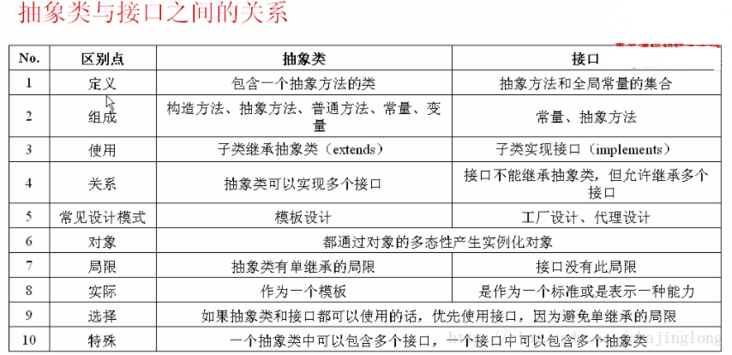
\includegraphics[width=.9\linewidth]{./pic/interface.png}

四种引用的区别

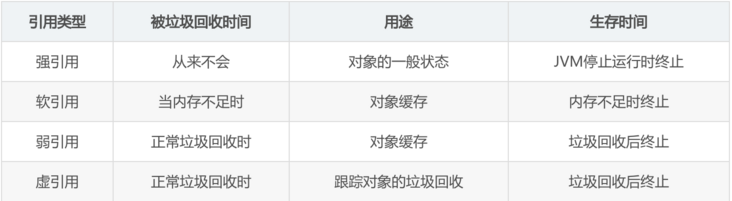
\includegraphics[width=.9\linewidth]{./pic/reference.png}

\begin{itemize}
\item \url{https://juejin.cn/post/7007326164268105741} 这个有没有时间看再说
\end{itemize}
% Emacs 27.1 (Org mode 8.2.7c)
\end{document}